\subsection{Interpreter}
\subsubsection{Định nghĩa}
Interpreter là một mẫu Pattern thuộc Behavioral Pattern cung cấp giải pháp để tạo ra đối tượng dựa trên mô tả người dùng trong lúc hoạt động chương trình. Nó thực thi một dòng lệnh hoặc một khối lệnh một cách tuần tự tại thời điểm chạy chương trình. Interpreter thực thi các dòng lệnh bằng cách chuyển nó thành mã máy cho phép chạy ngay lặp tức.
\subsubsection{Cách sử dụng}
Thông thương, ta hay sử dụng mẫu thiết kế trên trong các trường hợp:
\begin{itemize}
    \item Cho phép lập trình viên phát triển và hiện thực mã lệnh nhanh mà không cần phải complie. Sau mỗi lần chỉnh sửa mã nguồn, lập trình viên có thể chạy và xem kết quả ngay lặp tức.
    \item  Interpreter thường được sử dụng cho các ngôn ngữ có cấu trúc chạy từ trên xuống dưới như Python, Javascript,...
\end{itemize}
\subsubsection{Cấu trúc}
\begin{center}
    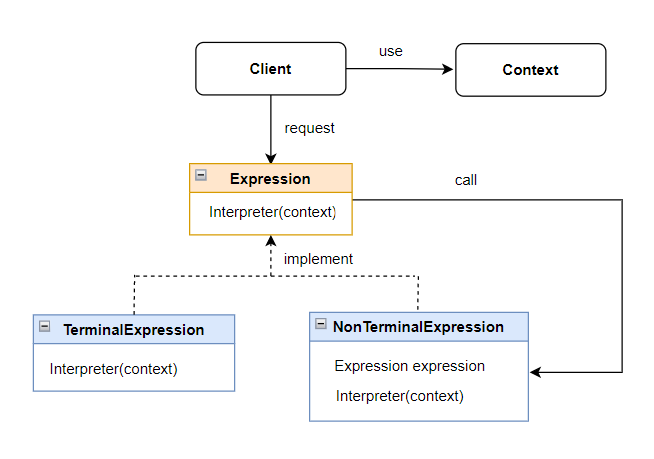
\includegraphics[scale= 0.6]{image/behavioral/interpreter.png}
\end{center}
Các thành phần chính của mẫu:
\begin{itemize}
    \item AbstractionExpression là một Class khai báo một giao diện cho việc thực thi một thao tác bất kì.
    \item TerminalExpression là một class cài đặt một thao tác thông dịch liên kết với những ký pháp đầu cuối, đóng vai trò một thể nghiệm được yêu cầu cho mọi ký pháp đầu cuối trong câu.
    \item NonterminalExpression là một class có thể chứa TerminalExpression bên trong và cũng có thể chứa một NonterminalExpression khác. Nó đóng vai trò như là “ngữ pháp” của ngôn ngữ đặc tả.
    \item Context: Là đối tượng thông tin để thực hiện thông dịch. Đối tượng này là toàn cục đối với quá trình thông dịch.
\end{itemize}
\subsubsection{Ưu điểm và Nhược điểm}
Có các ưu điểm và nhược điểm sau:
Ưu điểm:
\begin{itemize}
    \item Giảm số lượng những lớp con không cần thiết.
    \item Cho phép ẩn các chi tiết implement từ client.
    \item Vì không cần biên dịch trước, việc chỉnh sửa và chạy lại mã nguồn nhanh chóng.
    \item Interpreter có thể chạy trên nhiều nền tảng khác nhau mà không cần biên dịch lại.
\end{itemize}
Nhược điểm:
\begin{itemize}
    \item Interpreter phải dịch và thực thi từng dòng lệnh một tại thời điểm chạy, do đó tốn thời gian hơn so với việc biên dịch trước.
    \item Hiệu suất thấp.
    \item Đòi hỏi ngôn ngữ được xây dựng phải có cấu trúc đơn giản.
\end{itemize}

\subsubsection{Code Example}
\begin{itemize}
    \item Có một abtract class Expression để địng nghĩa dạng của kiểu lưu Expression.
    \item Các class Variable, Constant, Add, Subtract đại diện cho các biểu thức đại số (terminal và non-terminal) được kế thừa từ lớp Expresion ở trên.
\end{itemize}
\begin{lstlisting}
#include <iostream>
#include <string>
#include <unordered_map>

// Abstract Expression
class Expression {
public:
    virtual int interpret(std::unordered_map<char, int>& variables) = 0;
};

// Terminal Expression
class Variable : public Expression {
private:
    char variableName;
public:
    Variable(char name) : variableName(name) {}
    int interpret(std::unordered_map<char, int>& variables) override {
        return variables[variableName];
    }
};

// Terminal Expression
class Constant : public Expression {
private:
    int value;
public:
    Constant(int val) : value(val) {}
    int interpret(std::unordered_map<char, int>& variables) override {
        return value;
    }
};

// Non-terminal Expression
class Add : public Expression {
private:
    Expression* left;
    Expression* right;
public:
    Add(Expression* l, Expression* r) : left(l), right(r) {}
    int interpret(std::unordered_map<char, int>& variables) override {
        return left->interpret(variables) + right->interpret(variables);
    }
};

// Non-terminal Expression
class Subtract : public Expression {
private:
    Expression* left;
    Expression* right;
public:
    Subtract(Expression* l, Expression* r) : left(l), right(r) {}
    int interpret(std::unordered_map<char, int>& variables) override {
        return left->interpret(variables) - right->interpret(variables);
    }
};

// Client
int main() {
    std::unordered_map<char, int> variables;
    variables['x'] = 5;
    variables['y'] = 3;

    Expression* expression = new Subtract(
        new Add(new Variable('x'), new Variable('y')),
        new Constant(2)
    );

    int result = expression->interpret(variables);
    std::cout << "Result: " << result << std::endl;

    delete expression;

    return 0;
}


\end{lstlisting}
Trong phần main(), chúng ta khởi tạo các biến và xây dựng một biểu thức để tính toán (x + y - 2). Sau đó, chúng ta gọi hàm interpret() của biểu thức đó với một unorderedmap chứa giá trị của các biến (x = 5 và y = 3). Kết quả tính toán được in ra màn hình.
\\
\newline
\textbf{Kết quả:}
\begin{lstlisting}
Result: 6
\end{lstlisting}
\subsubsection{Các Pattern liên quan}
\begin{itemize}
    \item Composite là cây có trúc ngữ pháp trừu tượng
    \item Sử dụng Iterator để duyệt các dòng lệnh.
    \item Visitor có thể được sử dụng để duy trì hành vi trên mỗi nút trong cây cú pháp trừu tượng của lớp.
\end{itemize}